\documentclass{article}

\usepackage[utf8]{inputenc}
\usepackage{url}
\def\UrlFont{\em}
\usepackage{indentfirst}

\title{Trabalho de Visão Relatório}
\author{Felipe Leivas Machado - 262528 \and Priscila Cavalli Rachevsky - 261573 }

\usepackage{natbib}
\usepackage{graphicx}
\usepackage{capt-of}

\begin{document}

\maketitle

\section{Questão 1}
    Nesta questão precisavamos desenhar uma linha para representar um jogador que estaria num certo ponto \((x, y)\), onde \(x\) e \(y\) representam as cordenadas do pixel dos pés do jogador. Para podermos fazer isso precisavamos de algumas coisas, como:
   \begin{itemize}
       \item Coleta dos pontos de calibragem
       \item Descobrir matriz da câmera
       \item Converter uma coordenada 2D para uma cordenada 3D
       \item Converter uma coordenada 3D  para uma cordenada 2D
       \item Testar Matriz P
       \item Desenhar jogador
   \end{itemize}

    \subsection{Coleta dos pontos de calibragem}
        A coleta dos pontos na imagem foi feita manualmente, conforme Figure \ref{fig:maracana1Pontos} e depois calculados conforme a nova origem, já para acharmos os  respectivos  pontos  no  mundo  real, se usou a definição do trabalho com o tamanho do campo e da goleira.
        \begin{figure}[h!]
            \centering
            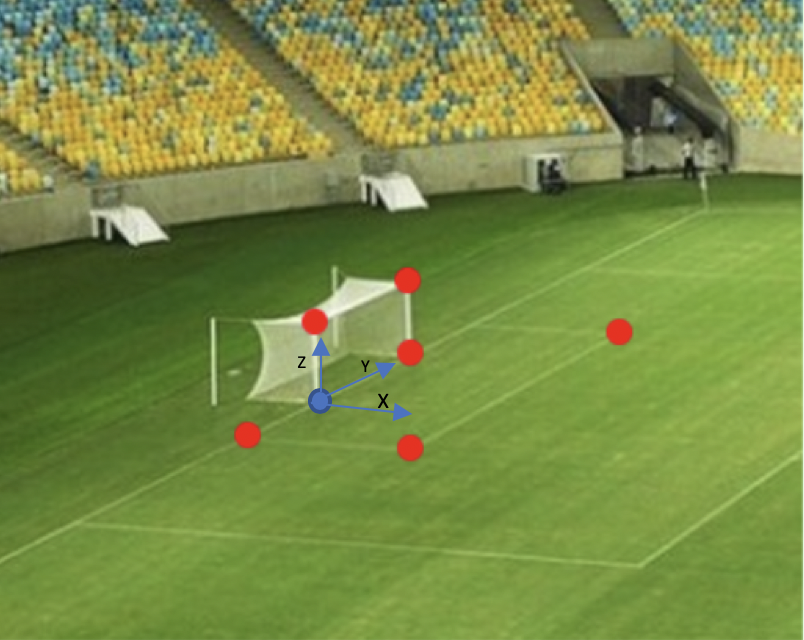
\includegraphics[scale=0.6]{maracana1Pontos.png}
            \caption{Em vermelho os 6 pontos escolhidos e em azul a origem}
            \label{fig:maracana1Pontos}
        \end{figure}

    \subsection{Descobrir matriz da câmera}
    Para descrobirmos a matriz de calibragem, primeiramente foi gerada a matriz A, conforme Figure \ref{fig:matrizA1}  com base nos 6 pontos selecionados. Depois foi feito um programa em python para obter os 12 coeficientes da matriz de projeção atrávez da decomposição SVD.
        \begin{figure}[h!]
            \centering
            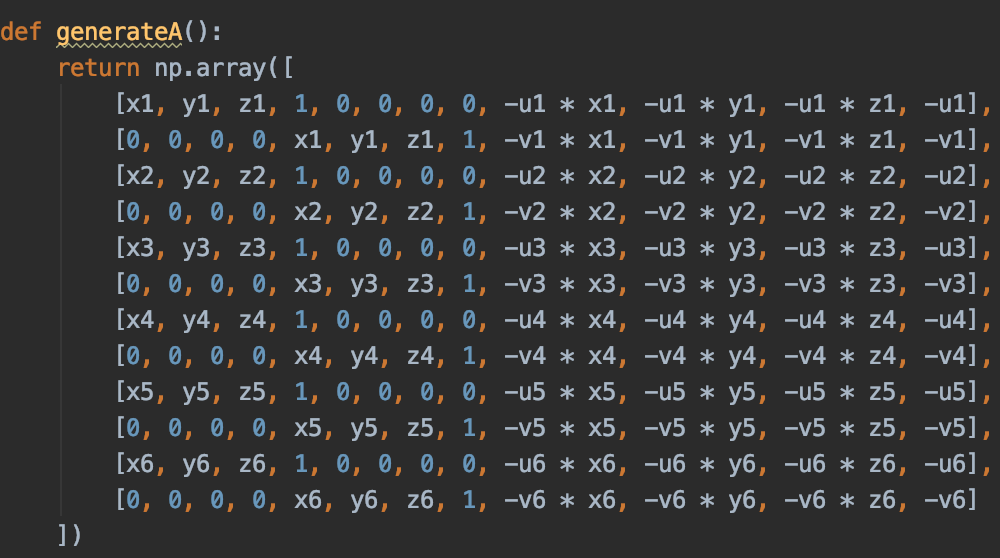
\includegraphics[scale=0.6]{matrizA1.png}
            \caption{Matriz A gerada com base nos 6 pontos}
            \label{fig:matrizA1}
        \end{figure}

    \subsection{Converter uma cordenada 2D para cordenada 3D}
    Para converter de um pixel para as cordenadas reais, depois de já ter a matriz de calibragem(P), foi preciso primeiro, escolher um dos planos para o ponto pertencer. Como o ponto selecionado sempre era nos pés do jogador, se disse que o \(z\) era sempre igual a 0. Então adaptamos a matriz P para ignorar os ponto do plano \(z\), removendo a 3ª coluna dela. Então foi só necessário obter a matriz inversa dessa nova matriz P, e multiplicar ela pelas cordenadas do pixel e depois conveter de cordenadas homogêneas para cordenadas  \((x, y)\).

    \subsection{Converter uma cordenada 3D para cordenada 2D}
    Para converter de um cordenadas reais para pixel, depois de já ter a matriz de calibragem, basta multiplicar a matriz P pelas cordenadas do mundo real.
    \subsection{Testar Matriz P}
    Para testarmos a matriz calculada P, pegamos alguns pontos  no mundo real conhecidos, que não foram utilizados para calcular a matriz P, e mapeamos para o pixel, para ver se eles eram iguais aos pixels na imagem. Como eles eram iguais assumimos que a matriz estava correta.
    \subsection{Desenhar jogador}
    Para desenharmos o jogador num certo pixel \(P_1\), primeiro precisávamos mapear esse pixel para cordenadas do mundo real, o jogador sempre está no chão, então assumimos \(z\)=0. Depois de obter a cordenada no mundo, geramos outro ponto \(P_2\), que seria a cabeça do jogador, essa ponto tinha todas suas cordenadas iguais a \(P_1\) mas com o \(z\)=1.8. Então depois de obtidos os dois pontos só desenhamos uma reta ligando esses dois pontos.
    \begin{figure}[h!]
    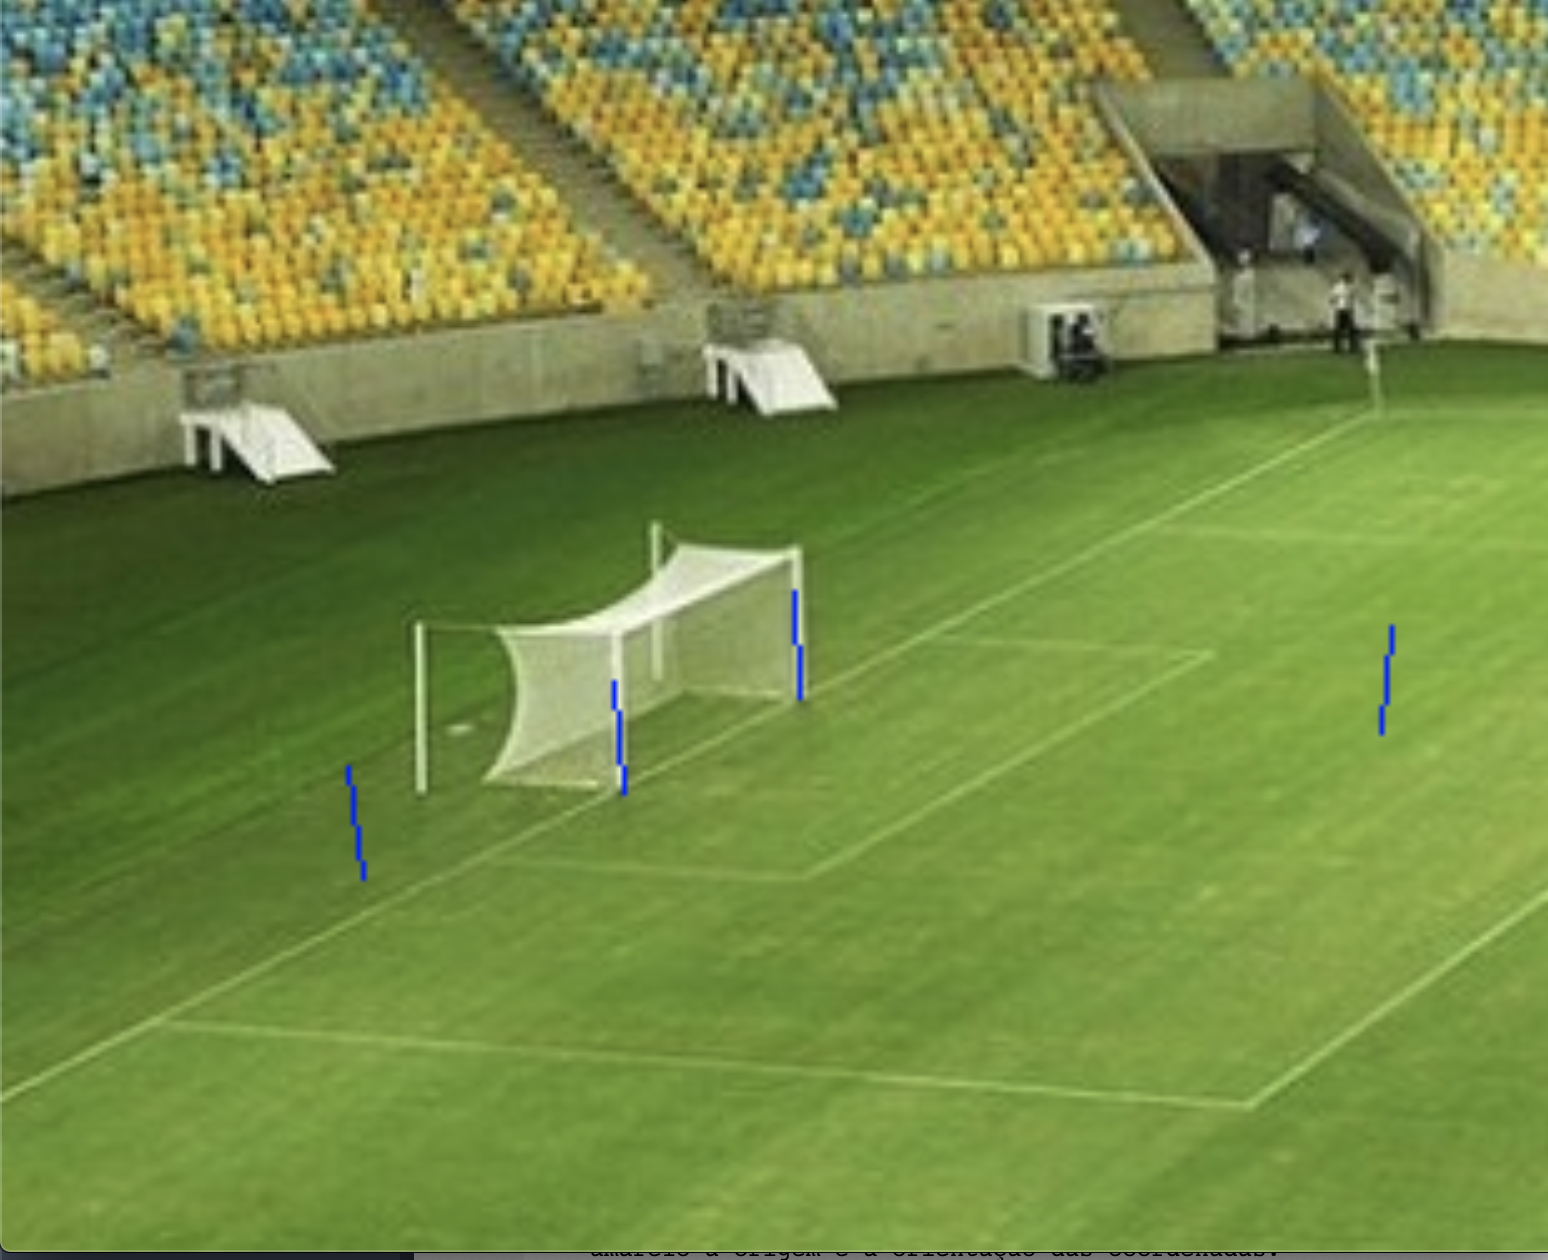
\includegraphics[scale=0.4]{jogadore1.png}
    \caption{Projeção dos jogadores pela matriz P}
    \label{fig:resultado1}
    \end{figure}
    \subsection{Resultado}
    Como podemos ver na Figure \ref{fig:resultado1} os jogadores projetados desenhados seguem a curvatura da lente, e estão alinhados com as traves. Então consideramos o resultado satisfatório.

\section{Questão 2}
    Desenhar uma linha no campo paralela à de impedimento, para isso foi necessário fazer os seguintes passos:
   \begin{itemize}
       \item Coleta dos pontos de calibragem
       \item Descobrir matriz da câmera
       \item Desenhar uma reta entre dois pontos
   \end{itemize}

    \subsection{Coleta dos pontos de calibragem}
    Foi feita da mesma forma que no exercício passado,porém ao contrário do exercício anterior, não foi preciso escolher pontos em que a coordenada \(z\) fosse diferente de 0, porque nesse exercício se usou estratégia de calibragem \textit{plane to plane}. Além disso provou-se que apenas 4 pontos já era o suficiente.

    Na Figure ~\ref{fig:maracana2Pontos} pode-se ver os 4 pontos escolhidos em vermelho, em amarelo a origem e a orientação das coordenadas.
        \begin{figure}[h!]
        \centering
        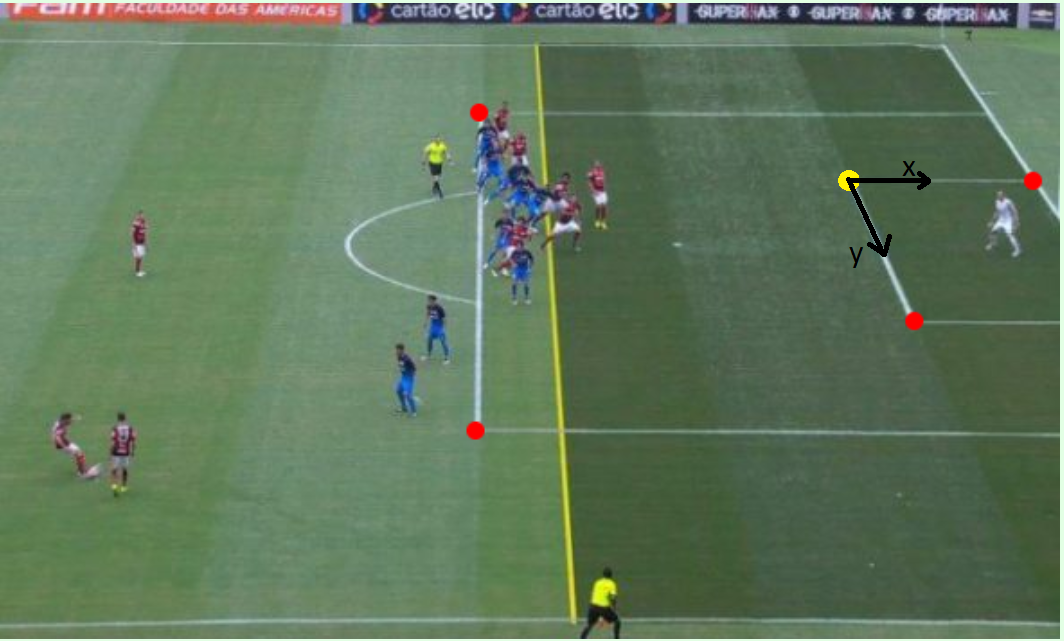
\includegraphics[scale=0.6]{maracana2Pontos.PNG}
        \caption{Em vermelho os 4 pontos escolhidos e em amarelo a origem}
        \label{fig:maracana2Pontos}
        \end{figure}

    \subsection{Descobrir matriz da câmera}
    Para descobrir a matriz da câmera deve-se descobrir a matriz P. Então, reutilizou as estratégia da questão anterior, modificando a equação como mostra a Figure ~\ref{fig:planeToPlane}.
    \begin{figure}[h!]
    \centering
    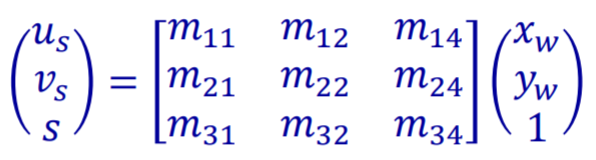
\includegraphics[scale=0.6]{planeToPlane.PNG}
    \caption{O modelo matemático para calibragem \textit{plane to plane}}
    \label{fig:planeToPlane}
    \end{figure}

        \subsubsection{Matriz A}
        A matriz A foi modificada para ter o tamanho 9x4, já que retirou-se as três colunas que eram associadas à coordenada \(z\) e usou-se apenas 4 pontos, como mencionado anteriormente. (Figure ~\ref{fig:matrizA})

        \begin{figure}[h!]
        \centering
        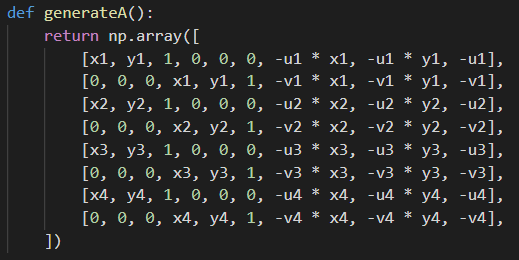
\includegraphics[scale=1]{matrizA.PNG}
        \caption{Matriz A para calibragem \textit{plane to plane}}
        \label{fig:matrizA}
        \end{figure}

        \subsubsection{Matriz P}
        Fez-se \textit{svd} na Matriz A, então pegou a última matriz de V e se fez o \textit{reshape} para ficar do tamnho \(3x3\). (Figure ~\ref{fig:matrizP})

        \begin{figure}[h!]         \centering
        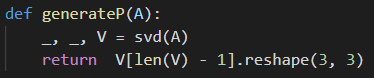
\includegraphics[scale=1]{matrizP.PNG}
        \caption{Matriz P a partir da matriz A}
        \label{fig:matrizP}
        \end{figure}

    \subsection{Desenhar uma reta entre uma lateral a outra}
    Tem diversas formas de desenhar linhas paralelas a do impedimento, nesse trabalho escolheu-se a solução em que desenhava uma reta de uma lateral a outra.

    Assim, só precisou descobrir os pontos das laterais. Implementou-se dessa forma: dado um ponto clicado na imagem e calculado no sistema 2D, descobria-se seu respectivo ponto \(P_m\) no mundo real (Figure ~\ref{fig:calculateRealWorldPoint}), e então, descobria os dois pontos em cada lateral (\(P_{11}\) e \(P_{12}\)) fazendo \(P_{11}\) = (\(P_m[x], Y_{lateralDeCima})\) e \(P_{12}\) = (\(P_m[x], Y_{lateralDeBaixo})\). Porém, a imagem da definição do trabalho não deixava claro qual o tamanho exato do campo (de 45 a 90m), então, também coletados manualmente, dois pixels localizados cada um em uma lateral e transformados em pontos do mundo real, então descobriu que a quadra tem aproximadamente 67m. Dessa forma, sabendo a origem, foi possível calcular o valor de \(Y_{lateralDeCima}\) e \(Y_{lateralDeBaixo}\).

        \begin{figure}[h!]
        \centering
        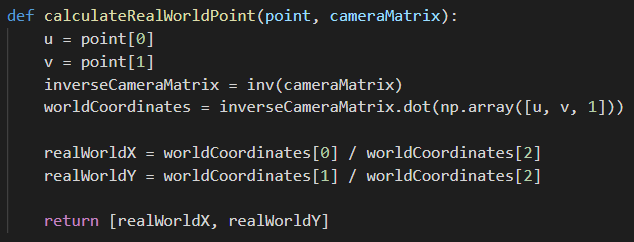
\includegraphics[scale=0.9]{calculateRealWorldPoint.PNG}
        \caption{Função que calcula o ponto no mundo real dado o ponto na imagem e a matriz da câmera}
        \label{fig:calculateRealWorldPoint}
        \end{figure}
    \subsection {Resultado}
    A Figure ~\ref{fig:result2} é o resultado do execício, pode se ver que não ficou perfeitamente paralelo a linha da pequena área, mas consideramos um resultado satisfatório.
        \begin{figure}[h!]
        \centering
        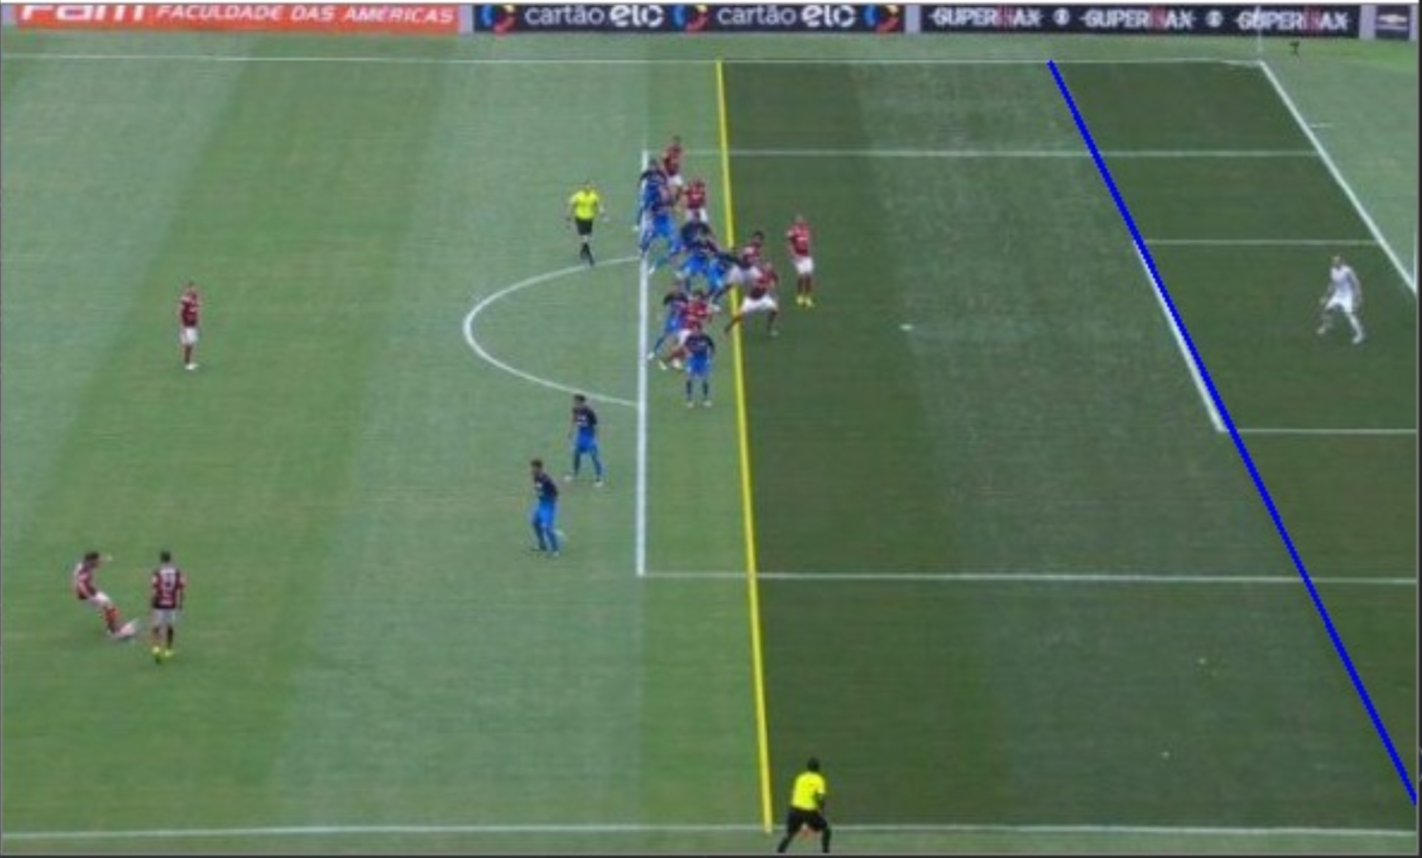
\includegraphics[scale=0.5]{result2.PNG}
        \caption{Função que calcula o ponto no mundo real dado o ponto na imagem e a matriz da câmera}
        \label{fig:result2}
        \end{figure}
\end{document}
